\chapter{Additional Controls for the Game-Based Experiments}\label{app:rebuttal-controls}

This appendix reports additional controls for the game-based attribution results in Section~\ref{sec:results_vit}. Benchmark configurations are selected on the 50-image validation split; test data do not enter selection. Fixed diagnostic choices are stated below. Held-out comparisons use paired image-bootstrap intervals.

\section{Sharpening and Full-Curve Faithfulness}\label{app:rebuttal-sharpening}

For a nonnegative spatial map $s$, the fixed sharpening transform is $s_i^{(p)}=s_i^p/\sum_j s_j^p$. At $p=1.5$ it preserves pixel order, and thus the deletion/insertion rankings of a fixed map, while changing magnitude-sensitive localization. The validation-matched control selects each LRP baseline by proximity of its validation AL to the predetermined RG AL; the test set is evaluated once. AttnLRP reaches test AL $0.715$ versus RG $0.711$ (paired difference $+0.004$, 95\% CI $[-0.007,0.015]$) and has lower PF$_{20}$, $6.123$ versus $7.481$. LRP-$\gamma$ reaches AL $0.694$ and PF$_{20}=6.398$. Thus the matched control does not support an RG localization--faithfulness Pareto advantage. This result is specific to the tested selection protocol and does not make post-hoc sharpening equivalent to internal routing changes.

\begin{table}[!ht]
\centering\small
\caption{Validation-matched fixed-$p=1.5$ sharpening on ViT-B/16. Baseline rows were selected by validation AL proximity to the fixed RG row. Differences and intervals are paired baseline minus RG over 565 test images; lower PF$_{20}$ is better.}
\label{tab:rebuttal-sharpening}
\begin{tabular}{lrrrr}
\toprule
Method & $p$ & Test AL & $\Delta$AL [95\% CI] & PF$_{20}$ \\
\midrule
RG (loc) & 1 & .711 & --- & 7.481 \\
LRP-$\gamma$ & 1.5 & .694 & $-.017\;[-.027,-.007]$ & 6.398 \\
AttnLRP & 1.5 & .715 & $+.004\;[-.007,+.015]$ & 6.123 \\
\bottomrule
\end{tabular}
\end{table}

Applying the same fixed $p=1.5$ to the AttnLRP, RG-anchor and localization-selected RG maps raises AL from $.6291$ to $.7153$, $.5093$ to $.5550$, and $.7112$ to $.7807$, respectively; each PF$_{20}$ remains unchanged because per-image pixel ranks are preserved. This common-power comparison is not AL-matched: the sharpened selected RG still has higher AL and worse PF$_{20}$ than AttnLRP. The exponent is fixed rather than selected, and the comparison does not claim optimality.

\begin{table}[!ht]
\centering\small
\begin{tabular}{lrrr}
\toprule
Method & AL, $p=1$ & AL, $p=1.5$ & PF$_{20}$ (unchanged) $\downarrow$ \\
\midrule
LRP-$\gamma$ & 0.6138 & 0.6942 & 6.3977 \\
AttnLRP & 0.6291 & 0.7153 & 6.1226 \\
RG anchor & 0.5093 & 0.5550 & 6.9673 \\
RG (loc) & 0.7112 & 0.7807 & 7.4807 \\
\bottomrule
\end{tabular}

\caption{Common fixed-$p=1.5$ map ablation on the same 565 ViT-B/16 test images. The exponent is applied after channel collapse, absolute-value reduction and max normalization; PF$_{20}$ is reused after per-image rank invariance was verified.}
\label{tab:rebuttal-common-power}
\end{table}

The separate full-curve control ranks $224^2$ spatial pixels by absolute attribution and perturbs all three RGB channels together. Deletion starts from the image; insertion starts from its per-channel spatial-mean image. The target is the dataset label, and the 101 cumulative fractions include both endpoints. This protocol differs from the benchmark PF$_5$/PF$_{20}$, which ranks channel-broadcast scalar features and integrates only an initial fraction. Under both raw-logit and probability AUC, the localization-selected LRP baselines outperform RG in both deletion and insertion direction; all eight paired baseline-versus-RG intervals exclude zero. Since the $p=1.5$ transform preserves pixel order, it also preserves these fixed-map curves.

\begin{table}[!ht]
\centering\scriptsize
\setlength{\tabcolsep}{3pt}
\resizebox{\linewidth}{!}{\begin{tabular}{lcccc}
\toprule
Method & Del. logit $\downarrow$ & Ins. logit $\uparrow$ & Del. prob. $\downarrow$ & Ins. prob. $\uparrow$ \\
\midrule
LRP-$\gamma$ (loc) & 3.111 [2.995, 3.229] & 7.778 [7.679, 7.872] & 0.128 [0.118, 0.137] & 0.617 [0.597, 0.635] \\
LRP-$\gamma$ (faith) & 3.124 [2.998, 3.250] & 7.531 [7.414, 7.646] & 0.126 [0.116, 0.137] & 0.579 [0.559, 0.599] \\
AttnLRP (loc) & 3.083 [2.961, 3.209] & 7.711 [7.601, 7.815] & 0.126 [0.116, 0.136] & 0.605 [0.585, 0.624] \\
AttnLRP (faith) & \textbf{2.962} [2.835, 3.091] & \textbf{7.909} [7.805, 8.009] & \textbf{0.115} [0.105, 0.125] & \textbf{0.634} [0.615, 0.653] \\
RG (loc) & 4.186 [4.045, 4.322] & 6.674 [6.544, 6.801] & 0.211 [0.196, 0.225] & 0.490 [0.471, 0.509] \\
RG (faith) & 3.164 [3.028, 3.304] & 6.870 [6.736, 6.997] & 0.142 [0.131, 0.153] & 0.500 [0.480, 0.520] \\
RG anchor & 3.146 [3.013, 3.277] & 7.021 [6.894, 7.146] & 0.146 [0.136, 0.157] & 0.518 [0.498, 0.538] \\
\bottomrule
\end{tabular}
}
\caption{Full spatial-pixel deletion and insertion AUC, ViT-B/16, $n=565$. Entries are means with image-bootstrap 95\% intervals. Lower deletion and higher insertion are favorable.}
\label{tab:rebuttal-full-auc}
\end{table}

\begin{figure}[!ht]
\centering
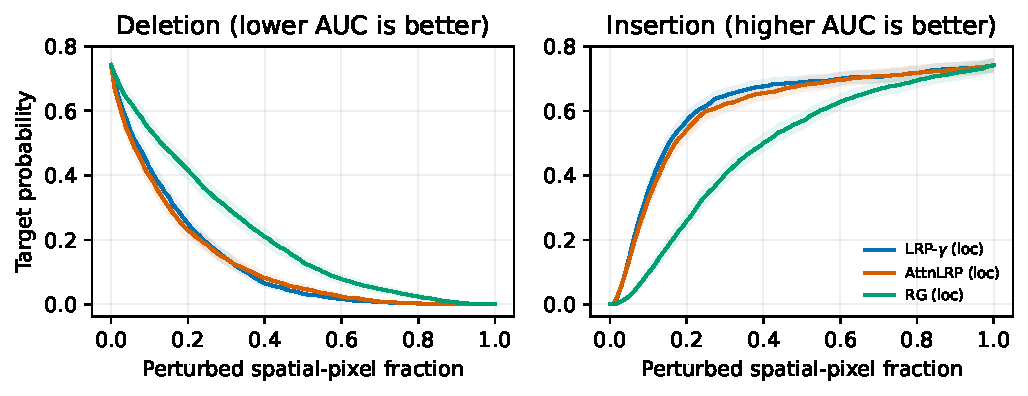
\includegraphics[width=.95\linewidth]{figures/rebuttal/full_auc_probabilities_selected.pdf}\\[.4em]
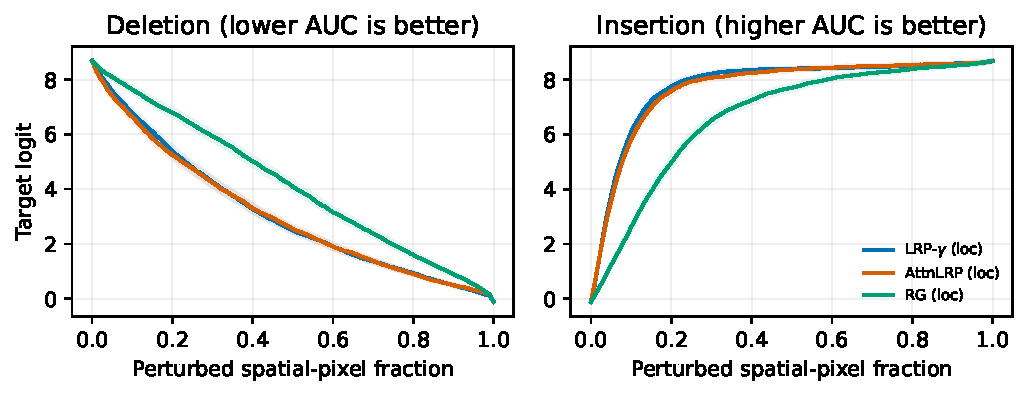
\includegraphics[width=.95\linewidth]{figures/rebuttal/full_auc_logits_selected.pdf}
\caption{Mean full deletion and insertion curves for localization-selected ViT-B/16 rows, using target probabilities (top) and raw target logits (bottom). Shading denotes pointwise image-bootstrap 95\% intervals.}
\label{fig:rebuttal-full-auc}
\end{figure}

\section{Robustness Controls}\label{app:rebuttal-robustness}

The ViT full-test robustness evaluation covers the validation-selected localization mode on all 565 images, using 50 image-keyed Uniform$[-0.2,0.2]$ perturbations in normalized input coordinates and 10,000 paired image resamples (seed 42). Validation selected $\lambda_{\mathrm{sm}}=-50$ at the fixed localization center. Compared with zero risk, MaxS changes from $.6850$ to $.6013$, AvgS from $.4447$ to $.3272$, while AL falls from $.6706$ to $.5204$. Thus lower sensitivity accompanies a substantial localization cost in this selected mode.

VGG-16 uses a gate-matched decomposition at the anchor. The first step changes a hard gate to a probit gate with $\lambda=0$; the second varies only $\lambda$ under that probit gate; the combined contrast compares the original hard-gate zero-risk row with the selected probit $\lambda=-2$ row. The table reports held-out means and paired differences, with 10,000 image-bootstrap resamples. The coefficient-only sensitivity gain incurs a small AL cost; the combined AL interval includes zero. This comparison isolates a selection-dependent effect and does not establish general robustness superiority.

\begin{table}[!ht]
\centering\small
\setlength{\tabcolsep}{4pt}
\begin{tabular}{>{\raggedright\arraybackslash}p{2.4cm}p{4.2cm}p{4.2cm}p{4.2cm}}
\toprule
Contrast & MaxS $\downarrow$ & AvgS $\downarrow$ & AL $\uparrow$ \\
\midrule
ViT loc, $\tau=.4,\varepsilon=.1$; $\lambda_{sm}:0\to-50$ & \shortstack{$.6850\to.6013$\\$\Delta=-.0837$\\$[-.1250,-.0419]$} & \shortstack{$.4447\to.3272$\\$\Delta=-.1176$\\$[-.1365,-.0985]$} & \shortstack{$.6706\to.5204$\\$\Delta=-.1502$\\$[-.1689,-.1322]$} \\
VGG anchor, gate only & \shortstack{$.5546\to.5265$\\$\Delta=-.0281$\\$[-.0330,-.0234]$} & \shortstack{$.4005\to.3714$\\$\Delta=-.0291$\\$[-.0317,-.0267]$} & \shortstack{$.6190\to.6207$\\$\Delta=+.0017$\\$[-.0002,+.0037]$} \\
VGG anchor, probit $\lambda:0\to-2$ & \shortstack{$.5265\to.4865$\\$\Delta=-.0400$\\$[-.0540,-.0264]$} & \shortstack{$.3714\to.3197$\\$\Delta=-.0518$\\$[-.0577,-.0460]$} & \shortstack{$.6207\to.6107$\\$\Delta=-.0100$\\$[-.0178,-.0021]$} \\
VGG anchor, combined & \shortstack{$.5546\to.4865$\\$\Delta=-.0680$\\$[-.0832,-.0532]$} & \shortstack{$.4005\to.3197$\\$\Delta=-.0808$\\$[-.0884,-.0737]$} & \shortstack{$.6190\to.6107$\\$\Delta=-.0083$\\$[-.0178,+.0013]$} \\
\bottomrule
\end{tabular}
\caption{Validation-selected risk contrasts on the full 565-image test set. Each cell gives both means, their difference (right minus left), and its paired 95\% interval. The ViT result is the selected localization-mode coefficient versus zero risk; VGG contrasts separate gate, coefficient and combined effects.}
\label{tab:rebuttal-risk}
\end{table}

The noise-protocol panel is a validation-only check of the ViT localization center ($n=50$). It crosses uniform and variance-matched Gaussian noise, $r\in\{.05,.1,.2\}$, and nested draw counts $\{10,25,50,100,200\}$, producing 30 correlated settings. For each setting, the risk-selected $\lambda_{sm}=-50$ is compared with zero risk using paired image intervals; intervals are unadjusted. MaxS, AvgS and 95th-percentile sensitivity means favor risk aversion in all 30 settings; their intervals exclude zero in 10, 30 and 19 settings, respectively. Cosine similarity favors risk aversion in all 30 settings, with intervals excluding zero in 10. Spearman similarity favors zero risk in all 30 settings, with intervals excluding zero in all 30. Top-10\% overlap means favor zero risk in all 30 settings, with intervals excluding zero in 10. Normalized-mass total variation favors risk aversion in 8 settings, with no interval excluding zero. These outcomes show that sensitivity and rank-based robustness diagnostics need not agree.

\section{Stopping-Game Pooling and Signed-Gradient Controls}\label{app:rebuttal-sg}

The submitted stopping-game (SG) benchmark exports the positive-player/positive-input (\texttt{pp}) component, not the signed occupation difference that recovers the input gradient. The original-forward pooling control caches max-pooling winners from the ordinary model forward and reuses them in the decomposed pass, keeping the submitted readout and all other settings fixed. On the 50-image VGG-16 validation split, the three configurations have identical PG, TK and Selectivity; paired intervals for AL, PF$_5$, PF$_{20}$, MaxS and AvgS contain zero except a $10^{-6}$ MaxS shift. This shows that pooling-index drift has negligible effect on the reported validation metrics at their precision. It is a diagnostic, not an equivalence test or a test-set result.

Separately, under per-layer numerical centering and cached original-forward pooling, the signed SG result matches autograd on all 50 validation images to a maximum relative $\ell_2$ error of $6.581\times10^{-7}$ with the theorem's strict ReLU-zero convention in float32; float64 reaches machine precision. The implementation's non-strict zero gate has larger float32 error ($2.873\times10^{-4}$ relative), while no exact-zero gate occurs in the float64 pass. Centering preserves the signed difference in exact arithmetic but changes individual components. This audit verifies the signed identity; it does not convert the submitted \texttt{pp} benchmark into a gradient benchmark.

\begin{table}[!ht]
\centering\small
\setlength{\tabcolsep}{3pt}
\begin{tabularx}{\linewidth}{>{\raggedright\arraybackslash}p{1.8cm}*{3}{>{\raggedright\arraybackslash}X}}
\toprule
Metric & Hard gate $\lambda=0$ & Localization-selected & Faithfulness-selected \\
\midrule
AL & \shortstack[l]{R/C: .5406/.5406\\$\Delta=-3.74\mathrm{e}{-07}$\\$[-1.46\mathrm{e}{-06},+4.31\mathrm{e}{-07}]$} & \shortstack[l]{R/C: .5681/.5681\\$\Delta=+4.04\mathrm{e}{-08}$\\$[-1.72\mathrm{e}{-07},+3.02\mathrm{e}{-07}]$} & \shortstack[l]{R/C: .5609/.5609\\$\Delta=+2.65\mathrm{e}{-08}$\\$[-3.34\mathrm{e}{-08},+1.20\mathrm{e}{-07}]$} \\
PG & \shortstack[l]{.7600/.7600\\$\Delta=+0.0000$\\$[+0.0000,+0.0000]$} & \shortstack[l]{.8800/.8800\\$\Delta=+0.0000$\\$[+0.0000,+0.0000]$} & \shortstack[l]{.7800/.7800\\$\Delta=+0.0000$\\$[+0.0000,+0.0000]$} \\
TK & \shortstack[l]{.7491/.7491\\$\Delta=+0.0000$\\$[+0.0000,+0.0000]$} & \shortstack[l]{.7306/.7306\\$\Delta=+0.0000$\\$[+0.0000,+0.0000]$} & \shortstack[l]{.7328/.7328\\$\Delta=+0.0000$\\$[+0.0000,+0.0000]$} \\
PF$_5$ & \shortstack[l]{17.396/17.395\\$\Delta=-0.002$\\$[-0.004,+4.37\mathrm{e}{-04}]$} & \shortstack[l]{16.339/16.341\\$\Delta=+0.001$\\$[-7.27\mathrm{e}{-05},+0.003]$} & \shortstack[l]{16.228/16.229\\$\Delta=+0.001$\\$[-0.001,+0.003]$} \\
PF$_{20}$ & \shortstack[l]{13.721/13.720\\$\Delta=-0.001$\\$[-0.002,+3.06\mathrm{e}{-04}]$} & \shortstack[l]{12.461/12.460\\$\Delta=-4.05\mathrm{e}{-04}$\\$[-0.001,+4.15\mathrm{e}{-04}]$} & \shortstack[l]{12.119/12.119\\$\Delta=+9.77\mathrm{e}{-05}$\\$[-0.001,+0.001]$} \\
Selectivity & \shortstack[l]{6.595/6.595\\$\Delta=+0.000$\\$[+0.000,+0.000]$} & \shortstack[l]{6.008/6.008\\$\Delta=+0.000$\\$[+0.000,+0.000]$} & \shortstack[l]{6.021/6.021\\$\Delta=+0.000$\\$[+0.000,+0.000]$} \\
MaxS & \shortstack[l]{.3758/.3758\\$\Delta=+6.69\mathrm{e}{-06}$\\$[-2.39\mathrm{e}{-06},+2.18\mathrm{e}{-05}]$} & \shortstack[l]{.2900/.2900\\$\Delta=+1.00\mathrm{e}{-06}$\\$[+2.01\mathrm{e}{-07},+1.96\mathrm{e}{-06}]$} & \shortstack[l]{.5315/.5315\\$\Delta=+3.69\mathrm{e}{-06}$\\$[-7.39\mathrm{e}{-06},+2.02\mathrm{e}{-05}]$} \\
AvgS & \shortstack[l]{.2845/.2845\\$\Delta=-1.28\mathrm{e}{-06}$\\$[-3.33\mathrm{e}{-06},+7.52\mathrm{e}{-07}]$} & \shortstack[l]{.1987/.1987\\$\Delta=+5.66\mathrm{e}{-07}$\\$[-2.68\mathrm{e}{-07},+1.51\mathrm{e}{-06}]$} & \shortstack[l]{.4180/.4179\\$\Delta=-2.01\mathrm{e}{-06}$\\$[-6.06\mathrm{e}{-06},+4.16\mathrm{e}{-07}]$} \\
$t$/img & \shortstack[l]{.074/.073\\$\Delta=-.001$\\$[-.002,-.001]$} & \shortstack[l]{.070/.074\\$\Delta=+.003$\\$[+.003,+.004]$} & \shortstack[l]{.070/.073\\$\Delta=+.003$\\$[+.003,+.003]$} \\
\bottomrule
\end{tabularx}

\caption{VGG-16 SG original-forward max-pooling control on the 50-image validation split. Each cell lists recompute/cached means followed by the paired cached-minus-recompute difference and its interval.}
\label{tab:rebuttal-sg-pooling}
\end{table}

\begin{changed}
\section{Routing-Game \texorpdfstring{$\alpha\beta$}{alpha-beta}-LRP Recovery}\label{app:rebuttal-rg}

We compare RG at $\tau=1$, with all policy deformations disabled, against independent $\alpha\beta$-LRP calculations. Each model uses three ImageNet-S validation images, $(\alpha,\beta)\in\{(1,0),(2,1)\}$ and $\varepsilon\in\{10^{-6},0.5\}$. A unit seed at the selected output logit fixes the relevance scale; errors compare the complete RGB relevance tensors before normalization or channel reduction. Bias shares are absorbed and each sign denominator receives its own $\varepsilon$, as in Theorem~\ref{ptnb:thm:ab-recovery}.

On pretrained VGG-16, the reference is Zennit's AlphaBeta rule, including signed first-layer contributions and ordinary max-pooling decisions. On pretrained ViT-B/16, an independent reverse recurrence covers the classifier, all twelve encoder blocks and the patch projection. It uses the observed QK-softmax, the composite Value rule of Theorem~\ref{ptnb:thm:attn-ab-recovery}, pass-through relevance at LayerNorm and GELU, and the implementation's full relevance to both addition operands (Section~\ref{ptnb:app:routing-skip}). Thus the ViT comparison verifies the stated local propagation rules throughout the model. Forward logits agree exactly on VGG-16 and within $7.11\times10^{-15}$ on ViT-B/16.

All end-to-end checks pass, reaching float64 relative errors below $3.3\times10^{-16}$ (Table~\ref{tab:rebuttal-rg-recovery}). Separately, fixed signed relevance seeds at each ViT attention--Value output test the composite rule in all twelve blocks: all 144 checks pass. These numerical checks use no reference-relevance injection and do not enter benchmark selection. Scripts, checkpoint hashes, image identifiers and per-run errors are retained with the code and in \nolinkurl{reports/evidence/routing-game-recovery/}.

\begin{table}[!ht]
\color{red}\centering\small
\begin{tabular}{llrrr}
\toprule
Model / scope & Precision & Checks & Max absolute error & Max relative $\ell_2$ error \\
\midrule
VGG-16 & float32 & 12 & $5.82\times10^{-10}$ & $4.11\times10^{-7}$ \\
VGG-16 & float64 & 12 & $4.34\times10^{-19}$ & $3.28\times10^{-16}$ \\
ViT-B/16 & float64 & 12 & $9.10\times10^{-13}$ & $3.19\times10^{-16}$ \\
ViT attention blocks & float64 & 144 & $5.26\times10^{-13}$ & $3.47\times10^{-14}$ \\
\bottomrule
\end{tabular}
\caption{RG recovery against independent $\alpha\beta$-LRP references on pretrained networks. Each entry is the worst error over the stated checks. End-to-end rows use unit output-logit seeds; the block row uses fixed signed relevance seeds.}
\label{tab:rebuttal-rg-recovery}
\end{table}
\end{changed}

\section{Checkpoint-Aligned Randomization and Local Hellinger Controls}\label{app:rebuttal-randomization}

The checkpoint-aligned ViT analysis evaluates map diagnostics and trajectory distance on the same 200 test images, dataset labels, model states and randomization conditions. Query/key/value projections remain pretrained in the cascade. Randomizing only the classifier head reduces top-1 accuracy from 88.5\% to zero and mean target probability from .7355 to .000932, while RG absolute-map rank similarity remains .999998; RG Hellinger distance is .769. Randomizing the last encoder block leaves map similarity at .999972 and raises Hellinger distance to .915. At the cascade endpoint, map similarity falls to .377 and survival-conditioned Hellinger reaches 1.000. The map projection can therefore remain nearly unchanged after predictive collapse, while the trajectory diagnostic registers changed routing. These results do not establish Hellinger as a predictor of accuracy or explanation quality.

Per-image associations are condition-dependent. At the cascade endpoint, RG Hellinger has Spearman correlation $-.203$ with RG map similarity (95\% CI $[-.333,-.072]$); head-only and last-block intervals include zero. The exploratory head-only association with absolute PF$_{20}$ change is $.273$ [$ .131,.403$], while other conditions include zero. Because randomization changes the classifier and logit scale, PF$_{20}$ change is not an independent explanation-quality endpoint. Local perturbations of the ViT classifier head produce increasing Hellinger distance as noise scale grows, while a small last-block attention-output perturbation produces much smaller distance; this is a local sensitivity diagnostic, not a quality calibration. Chapter~\ref{ch:trajectory} supplies the trajectory-space definitions and theorem scope.

\begin{table}[!ht]
\centering\scriptsize\setlength{\tabcolsep}{2pt}
\resizebox{\linewidth}{!}{\begin{tabular}{lrrrr}
\toprule
Condition & Top-1 acc. & Mean $p(y)$ & RG map $\rho(|a|)$ & $\mathrm{H}_{\mathrm{RG}}$ \\
\midrule
Identity & $88.5\%$ & $0.735504$ & $1.000000$ & $0.000$ \\
Head only & $0.0\%$ & $0.000932$ & $0.999998$ & $0.769$ \\
Last block & $0.0\%$ & $0.001016$ & $0.999972$ & $0.915$ \\
Cascade endpoint & $0.5\%$ & $0.000846$ & $0.377042$ & $0.963$ \\
\bottomrule
\end{tabular}
}
\caption{Prediction audit for the checkpoint-aligned ViT randomization controls ($n=200$ fixed test images).}
\label{tab:rebuttal-vit-prediction}
\end{table}

\begin{table}[!ht]
\centering\small\setlength{\tabcolsep}{3pt}
\begin{tabular}{@{}lccc@{}}
\toprule
Diagnostic & Head only & Through last block & Cascade endpoint \\
\midrule
Top-1 accuracy & $0.0\%$ & $0.0\%$ & $0.5\%$ \\
Mean target probability & $0.001$ & $0.001$ & $0.001$ \\
\midrule
\ac{sg}: $\mathrm H$ & $0.755\pm0.010$ & $0.886\pm0.004$ & $0.951\pm0.002$ \\
\ac{sg}: $\mathrm H_{\mathrm{surv}}$ & $0.755\pm0.010$ & $0.894\pm0.004$ & $1.000\pm0.000$ \\
\ac{rg}: $\mathrm H$ & $0.769\pm0.013$ & $0.915\pm0.005$ & $0.963\pm0.001$ \\
\ac{rg}: $\mathrm H_{\mathrm{surv}}$ & $0.770\pm0.013$ & $0.904\pm0.006$ & $1.000\pm0.000$ \\
\midrule
Gradient map $\rho(|a|)$ & $0.658\pm0.074$ & $0.655\pm0.074$ & $-0.035\pm0.134$ \\
\ac{rg} anchor map $\rho(|a|)$ & $1.000\pm0.000$ & $1.000\pm0.000$ & $0.377\pm0.238$ \\
\midrule
Association of \ac{rg} $\mathrm H$ with \ac{rg} map $\rho(|a|)$ & \shortstack{$+0.132$\\$[-0.010,+0.266]$} & \shortstack{$+0.059$\\$[-0.085,+0.199]$} & \shortstack{$-0.203$\\$[-0.333,-0.072]$} \\
\bottomrule
\end{tabular}

\caption{Checkpoint-aligned ViT map and trajectory diagnostics ($n=200$), transposed by diagnostic for legibility. Spearman associations are exploratory and unadjusted.}
\label{tab:rebuttal-vit-randomization}
\end{table}

\begin{table}[!ht]
\centering\small
\begin{tabular}{lrr}
\toprule
Perturbed module & Noise scale $s$ & $\mathrm{H}_{\mathrm{RG}}$ [95\% CI] \\
\midrule
Classifier head & $0.001$ & $0.001$ $[0.001,0.001]$ \\
Classifier head & $0.01$ & $0.011$ $[0.011,0.011]$ \\
Classifier head & $0.1$ & $0.090$ $[0.088,0.091]$ \\
Classifier head & $1$ & $0.500$ $[0.495,0.505]$ \\
Last-block attention output & $0.001$ & $0.001$ $[0.001,0.001]$ \\
\bottomrule
\end{tabular}

\caption{Local Hellinger response to controlled ViT weight perturbations.}
\label{tab:rebuttal-local-hellinger}
\end{table}

